\chapter{ISBI Challenge 2013}
\section{Introduction}
The goal of the ISBI Challenge, as announced on their website (\cite{challenge}), is to give an overview and understanding of availible algorithms for single particle localization microscopy. The focus was on 2d localisation, to give information about the depth of a localisated spot was optional. To benchmark results one needs groundtruth. Therefore the organisers created synthetic datasets of biologically relevant structures such as tubulins. To match realistic conditions the data was transformed to introduce different kinds of noise and background to it.\newline
The participants were given training data sets and the corresponding groundtruth and one month before the deadline of the challenge the test sets. There were two different kind of datasets in principle. One with very dense spots and shorter sequences, the other with longer sequences and fewer spots per frame.\newline
All paricipants were asked to submit their results and also the time it took to run the algorithm and the hardware configuration of the used system.

\section{Terminology}
To be able to compare different algorithms there must be a way to determine the correctly detected spots. To do so for each estimated positon of a flourophor, the nearest correct position of the molecule in the groundtruth data was searched within a lateral tolerance disc. Once a match was found this two spots were taken out of consideration for the matching.\newline
One important parameter for this evaluation is the radius of the lateral tolerance disk, because it has big influence on the number of detections considered to be true positives (TP).\newline
Detections with no associated spot in the groundtruth are called false positives (FP), spots in the groundtruth with no matching detection are called false negatives (FN).\newline
This matching is done frame by frame, it is not possible to match a point from different frames even if the $x$ and $y$ coordinates match perfectly but the frame differs.\newline
The precision ($p$) of a classification task is defined as the ration between the number of true positives and the sum of true positives and false positives:
\begin{equation}
\text{precision: }p = \frac{\text{TP}}{\text{TP}+\text{FP}} 
\end{equation}
It is a number between 0 at worst and 1 at best, telling how reliable the result is, how likely it is that a labeld sample really belongs to the predicted class. In this context it means how certain a detected spot has its origin in a fluorophore attached to the investigated structure and it's origin is not wrongly detected background noise.\newline
An other important value is the recall $r$ that is defined as the ratio of true positives and the sum of true positives and false negatives:
\begin{equation}
\text{recall: }r = \frac{\text{TP}}{\text{TP}+\text{FN}}
\end{equation}
The recall lies also in a range from 0 to 1  and gives an impression on how many relevant spots were found.

\section{Measures} 
For the evaluation three different measures were used. The f-score index $f$, the Jaccard index $J$ and the rot-mean square distance RSME. 
\begin{eqnarray}
	\text{f-score: }f &=\frac{2\cdot p \cdot r}{p+r} 
\end{eqnarray}
\subsection{Jaccard index}
Let $A$ be the set of points of the groundtruth and $B$ be the set of detected points. The Jaccard index $J$ is defined as:
\begin{equation}
\text{Jaccard: }J = \frac{\left|A\cap B\right|}{\left|A\cup B\right|}
\end{equation}
The intersection is done frame by frame. This means two spots from the groundtruth and the detection set just match if they occure in the same frame. 
\subsection{RSME}
The root-mean square distance gives an impression how big the squared distance between a spot in the groundtruth and an associated detection was in average. It can be calculated like this:
\begin{equation}
\text{RSME} = \frac{1}{\left|A\cap B\right|}\sum\limits_{i=1}^{\left|A\cap B\right|} \left(p_a(x,y)-p_b(x,y)\right)^2
\end{equation}
\section{Trainingsdata}
\subsection{Bundled tubes datasets}
There was two kinds of bundled tubes data sets, both created from the same underlying structure, one set with a high spot density and a short sequence of 360 frames, the other with fewer spots per frame but 12000 frames in total. Picture \ref{bundledtubesHighowDensityFrame} shows one frame of each data set.\newline
\begin{figure}
\begin{minipage}[t]{0.60\textwidth}
\subfloat[High spot density]{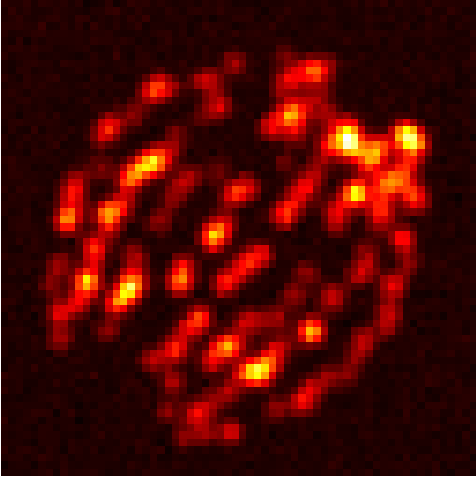
\includegraphics[width = 0.485\textwidth]{pictures/bundledTubesHighDensityFrameFarbig.png}}\hfill
\subfloat[Low spot density]{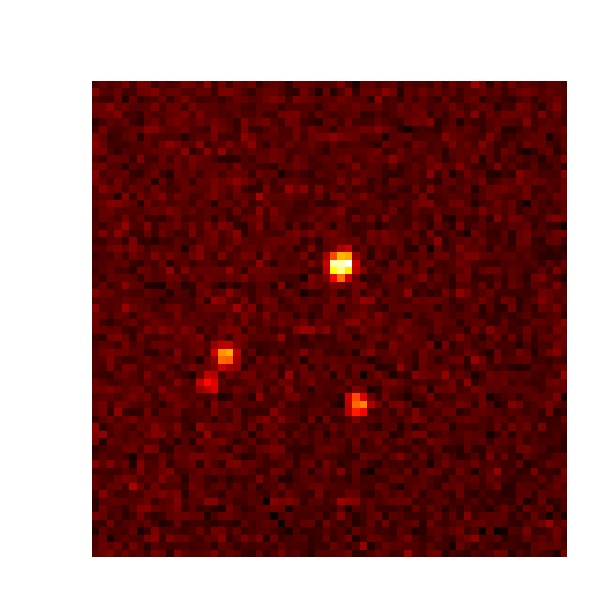
\includegraphics[width = 0.485\textwidth]{pictures/bundledTubesLowDensityFrameFarbig.png}}
	\caption{One frame from bundled tubes training data set}
	\label{bundledtubesHighowDensityFrame}	
\end{minipage}\hfill
\begin{minipage}[t]{0.33\textwidth}
\centering
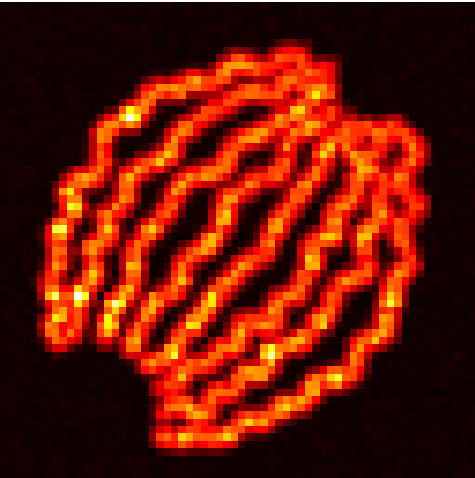
\includegraphics[width = 0.88\textwidth]{pictures/maximumProjectionBundledTubesLSFarbig.png}
	\caption{Maximum projection of bundled tubes data set}
	\label{pctMaximumProjBundledTubes}

\end{minipage}
\end{figure}
The original images very small, just 64 pixels in each dimension. Both sequences had spatial and temporal constant background. Picture \ref{pctMaximumProjBundledTubes} shows the maximum projection of the bundled tubes data set. The maximum projection is used to reduce the dimensionality of a data set. In this case for each pixel in $x$- and $y$-dimension, in the three dimensional dataset, the brightes value from all frames is taken. 


\subsection{Tubulin data sets}
The other training data sets models 7 microtubules, a structure that is a long filament up several micrometers long and a diameter of about 25 nanometers. The spot density lies somewhere between the high density and the low density of the bundled tubes data sets. This data sets show strong inhomogeneity in spatial dimensions and moderate inhomogeneity in temporal dimension, see figure \ref{tubulinVariableBg}. This is the reason why in the lower left corner of the maximum projection \ref{pctMaximumProjTubulin} a brighter area can be seen.

\begin{figure}
\subfloat[Tubulin2 frame 10]{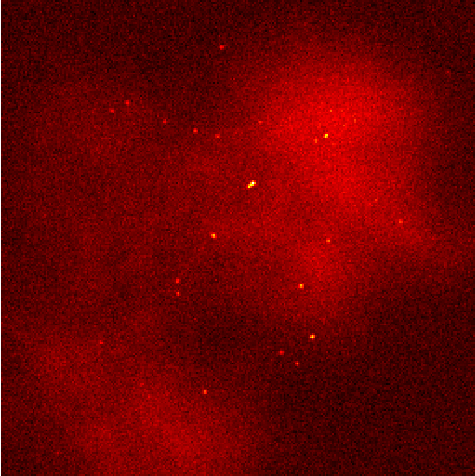
\includegraphics[width = 0.485\textwidth]{pictures/Tubulin2Frame10.png}}\hfill
\subfloat[Tubulin2 frame 1010]{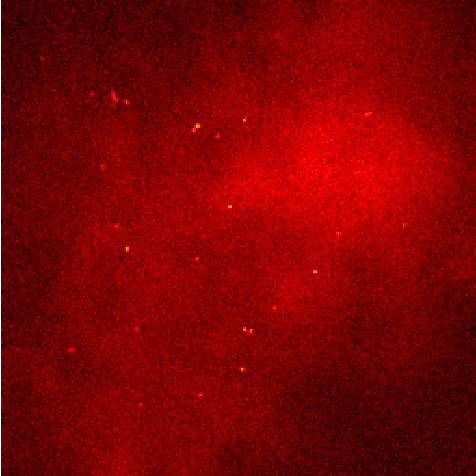
\includegraphics[width = 0.485\textwidth]{pictures/Tubulin2Frame1010.png}}
	\caption{This pictures show the variability of the background in the spatial and temporal dimensions}
	\label{tubulinVariableBg}	
\end{figure}

\begin{figure}
\centering
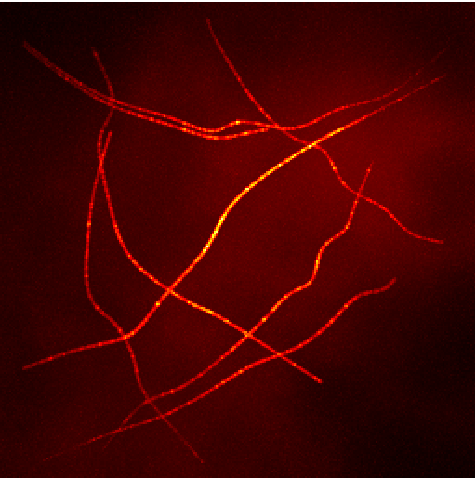
\includegraphics[width = 0.88\textwidth]{pictures/maximumProjectionTubulinFarbig.png}
	\caption{Maximum projection of tubulin data set}
	\label{pctMaximumProjTubulin}


\end{figure}

\section{Submissions}
\subsection{High precision}
\subsection{High score}
\subsection{Highest score via postprocessing}
\section{Results}